\chapter{Symulacja Software in the Loop}
\label{cha:symulacja}

% w tym rozdziale też jakieś screeny, wykresy, parametry itp.
% przebieg testów wraz z uzasadnieniem i komentarzem odnośnie wyników itp.

Pierwszym elementem, który w ramach projektu należało stworzyć, jest symulacja SiL (ang. \textit{Software in the Loop}). Celem jest otrzymanie narzędzia, które pozwoli na wygodne i~szybkie testowanie tworzonego w późniejszym etapie algorytmu detekcji przeszkód.

Przed przystąpieniem do realizacji zadania, warto zdefiniować wymagania i~oczekiwania, jakie są postawione przed gotowym oprogramowaniem:
\begin{enumerate}
    \item Symulacja powinna umożliwić testowanie dla różnych scenariuszy (np. inne przeszkody w~zmiennych pozycjach).
    \item W symulacji należy umieścić robota/drona, wyposażonego w~odpowiednie czujniki, z~których dane powinny być łatwo dostępne.
    
    Jako pojazd przenoszący kamerę zdarzeniową, dla którego będą wykrywane przeszkody, został wybrany czterowirnikowy dron. Taka decyzja uwarunkowana była kilkoma czynnikami:
    \begin{itemize}
        \item Zachowana zostaje analogia do analizowanych w~ramach przeglądu literatury projektów, w~których również wykorzystywano podobny pojazd. Ułatwia to wzorowanie się na zastosowanych w publikacjach metodach. 
        %Ułatwia to porównanie niniejszej pracy z publikacjami z literatury.
        \item Dron ma szerokie możliwości unikania wykrytych przeszkód, a~więc pełnego wykorzystania dostarczonych mu przez algorytm danych. Dzięki temu możliwości pojazdu nie będą ograniczeniem dla efektywności algorytmu sterującego, korzystającego z~informacji o~przeszkodach.
    \end{itemize}
    \item Użytkownik powinien mieć możliwość sterowania (za pomocą napisanego kodu) robotem/dronem poruszającym się po scenie symulacji.
    \item Symulacja powinna dostarczać dane z~kamery zdarzeniowej, umieszczonej na robocie/dronie.
\end{enumerate}



\section{Symulacja w Gazebo}
\label{sec:sym_gazebo}

Jako środowisko symulacyjne, w~którym całość została zrealizowana, wybrano oprogramowanie Gazebo.

% Jakbym chciał, żeby tu było więcej stron, to można jakieś loga tych narzędzi powrzucać czy jakieś scrreny przykładowe
% O Gazebo, Co to? Można potem przeniść do teorii

\textbf{Gazebo} jest otwartoźródłowym symulatorem robotyki, wykorzystywanym do testowania i~rozwijania algorytmów sterowania robotami w~realistycznym, trójwymiarowym środowisku. Zapewnia dostęp do zaawansowanego modelu fizyki oraz wielu czujników. Jest zintegrowany z~platformą programistyczną ROS2. Gazebo umożliwia umieszczanie na scenie zarówno obiektów statycznych, jak i~ruchomych. % -- taką rolę mogą pełnić na przykład chodzący szybkim krokiem ludzie.
Symulator pozwala też na stworzenie nocnej sceny.

\vspace{11px}
% Dlaczego gazebo
\noindent Oprócz wspomnianych funkcjonalności, Gazebo jest środowiskiem, które świetnie nadaje się do zastosowania w~projekcie z~dwóch głównych powodów:
\begin{itemize}
    \item Gazebo jest wspierane przez inne narzędzia, których użycie jest konieczne; w~szczególności ważna jest możliwość użycia wykorzystywanego w~projekcie narzędzia do sterowania lotem drona w~symulacji,
    \item Gazebo wykorzystuje i~wspiera użycie \textit{frameworka} ROS2, który jest konieczny do sterowania dronem oraz odczytywania danych z~czujników.
\end{itemize}

% O PX4

W celu umieszczenia w symulacji drona oraz zapewnienia możliwości sterowania nim należy wykorzystać odpowiednie oprogramowanie. Do tego celu wybrany został system \textbf{PX4 Autopilot}. Jest to zaawansowane, \textit{open-source}'owe oprogramowanie sterujące dla bezzałogowych statków latających (ale również dla innych robotów mobilnych). Jest jednym z najczęściej wykorzystywanych systemów autopilota w dziedzinie robotyki powietrznej i autonomicznych pojazdów, wspieranym przez aktywną społeczność i dużą liczbę integracji z różnorodnym sprzętem. Najważniejszymi dla projektu zaletami tego systemu są:
\begin{itemize}
    \item Wsparcie dla czterowirnikowych dronów,
    \item Możliwość sterowania za pomocą zewnętrznego oprogramowania, wykorzystując ROS2 -- tryb Offboard.
\end{itemize}

% O ROS2 - coś więcej o ROSie można potem dopisać w teorii - wyjąsnić jak działają węzły, topici i message, wtedy tu można skrócić



% Jak spełniłem kolejne wymagania z listy 
% \vspace{11px}
% \noindent \textbf{Realizacja}
% \vspace{11px}
\subsection{Przygotowanie środowiska}

Pierwszym krokiem realizacji symulacji była instalacja i przygotowanie środowiska. Dla systemu Linux w dystrybucji Ubuntu 22.04 pobrane zostały:
\begin{itemize}
    \item ROS2 w dystrybucji Humble,
    \item Symulator Gazebo,
    \item Python 3.10.
\end{itemize}

% Stworzenie świata w gazebo - konfiguracja z ROSem i PX4, wykorzytsanie gotowego przykładu - spełnienie wymagania 2 i 3

W celu umieszczenia drona w środowisku symulacyjnym i umożliwienia sterowania nim, wykorzystany został system PX4 Autopilot. Należy go odpowiednio skonfigurować do pracy z Gazebo i ROS-em, tak żeby było możliwe pisanie własnych węzłów (ang. \textit{node}) w Pythonie. Są to procesy, których zadaniem będzie na przykład sterowanie dronem lub przetwarzanie danych z czujników.

Ponieważ konfiguracja wszystkich narzędzi, tak by skutecznie ze sobą współpracowały, jest zadaniem stosunkowo trudnym -- szczególnie dla nowego użytkownika, warto skorzystać z gotowego przykładu i~dołączonej do niego instrukcji konfiguracji. Dzięki temu, dopóki dokładnie wykonuje się opisane kroki, zyskuje się względną pewność, że błędy popełnione na tym etapie nie utrudnią realizacji zadania w~przyszłości. Taki przykład dostępny jest na Githubie pod linkiem: \url{https://github.com/ARK-Electronics/ROS2_PX4_Offboard_Example}. Autorzy tego projektu poprawnie skonfigurowali go i~przygotowali do dalszej rozbudowy dla innych użytkowników.

Zawarte w przykładzie funkcjonalności obejmują:
\begin{itemize}
    \item Podstawowa, pusta scena w symulatorze Gazebo z umieszczonym w~niej czterowirnikowym dronem dostępnym w PX4 Autopilot,
    \item Przykład sterowania dronem, w~którym jako wartość zadana używany jest wektor prędkości -- na tej podstawie nowemu użytkownikowi łatwiej jest stworzyć własny system sterowania,
    \item Zaimplementowane zostało sterowanie kierunkiem i prędkością ruchu drona za pomocą strzałek na klawiaturze -- ta funkcjonalność nie jest wymagana w projekcie, jednak jest ciekawym przykładem, na podstawie którego można rozbudowywać symulację,
    \item Dodatkowy moduł wizualizacji, wykorzystujący narzędzie \textit{rviz}, służący do wyświetlenia ścieżki, jaką dron przebył w czasie trwania symulacji -- ten moduł również nie jest niezbędny, ale stanowi interesujący dodatek,
    \item Uruchamianie wszystkich modułów symulacji za pomocą jednej komendy, co znacząco ułatwia późniejsze z niej korzystanie.
\end{itemize}

Po dostosowaniu przykładu do zastosowania w projekcie, otrzymuje się gotową do dalszej pracy platformę, w której możliwe jest kontrolowanie drona za pomocą kodu pisanego w języku Python oraz obsługa danych z czujników.

Model drona wykorzystywany w symulacji to x500 (rys. \ref{fig:x500}) (nazwa używana w dokumentacji PX4). Jest on wyposażony w czujnik IMU (ang. \textit{inertial measurement unit}), który składa się z akcelerometru i żyroskopu i dostarcza danych o ruchu i orientacji drona w przestrzeni, niezbędnych do skutecznego sterowania nim.

% Screen drona

\begin{figure}
    \centering
    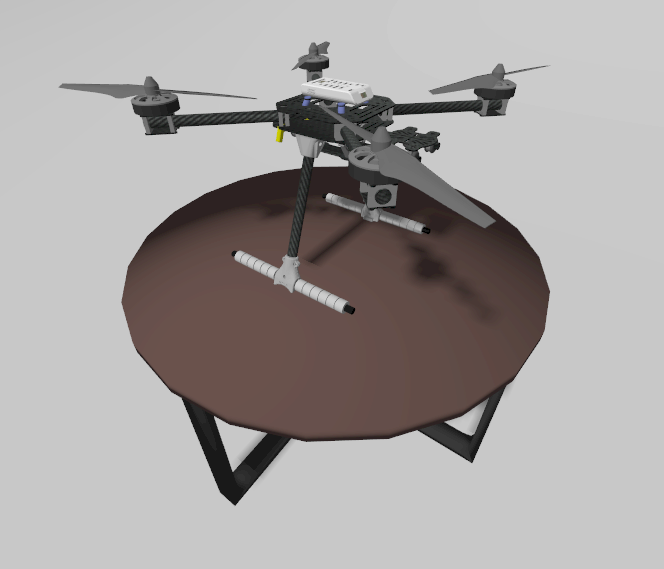
\includegraphics[width=0.5\linewidth]{images/x500.png}
    \caption{Model drona x500, dostępny w PX4 w symulacji w środowisku Gazebo.}
    \label{fig:x500}
\end{figure}

% Wymaganie 1 - losowe generowanie toru przeszkód
% \vspace{11px}
% \noindent \textbf{Losowe generowanie toru przeszkód}
% \vspace{11px}

\subsection{Losowe generowanie toru przeszkód}
\label{subsec:tor}

Dron powinien móc poruszać się w~scenie zawierającej statyczne przeszkody, które mógłby wykrywać i~omijać. 
W celu zapewnienia zmiennych warunków, w~jakich algorytm będzie testowany, należy stworzyć losowo generowany tor przeszkód. Żeby to osiągnąć, przygotowano odpowiedzialny za to skrypt w Pythonie.

Świat symulacji w~Gazebo generowany jest na podstawie kodu zawartego w~pliku \textit{.sdf}. To w~nim definiuje się używane pluginy (czyli moduły odpowiedzialne za różne zadania), czujniki, a~także umieszcza obiekty i~decyduje o~ich położeniu. Skrypt generujący przeszkody uruchamia się za każdym razem, gdy włączana jest symulacja, i~umieszcza obiekty w odpowiednim miejscu w kodzie w pliku \textit{.sdf}.

\vspace{11px}

Działanie skryptu generującego przeszkody:
\begin{itemize}
    \item Przekazanie parametrów wejściowych:
    \begin{itemize}
        \item Liczba przeszkód,
        \item Lista nazw przeszkód -- wybór z~trzech dostępnych: drzewo iglaste, drewniany słup energetyczny, szeroki cylindryczny słup,
        \item Obszar, który ma być pokryty przeszkodami,
        \item Minimalny dystans między dwoma obiektami,
    \end{itemize}
    \item Losowe wygenerowanie pozycji i~orientacji dla każdej przeszkody, tak by zachowany był minimalny dystans między nimi,
    \item Odpowiednie sformatowanie tekstu i~wpisanie go do pliku \textit{.sdf}.
\end{itemize}

Oprócz przeszkód w~symulacji umieszczony został jeszcze stolik -- stanowisko startowe dla drona, oraz bramka oznaczająca metę -- cel trasy drona.
Wszystkie wykorzystane obiekty pochodzą z~szerokiej biblioteki modeli dostępnych za darmo dla Gazebo: Gazebo Fuel. Łatwo dostępne modele dostosowane do szybkiego użycia w~symulacji to kolejna z zalet tego środowiska.

Dodatkowo można symulować ograniczone warunki oświetleniowe przez ręczne zmiany intensywności oświetlenia w~pliku \textit{.sdf}. 

Przykładowe sceny można zobaczyć na rysunku \ref{fig:sceny}.

% Może taki ładny screen z modelami przykładowych statycznych przeszkód, jak po prostu stoją obok siebie
% \begin{figure}
%     \centering
%     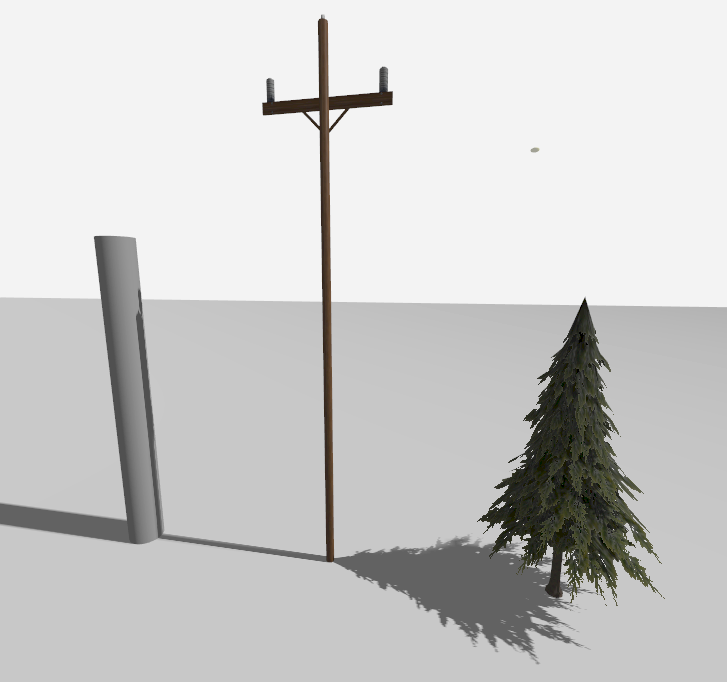
\includegraphics[width=0.5\linewidth]{images/obstacles.png}
%     \caption{Obiekty, które mogą zostać umieszczone na trasie drona, pozyskane z biblioteki Gazebo Fuel.}
%     \label{fig:obiekty}
% \end{figure}

% Ze dwa screeny sceny
\begin{figure}
    \centering
    \begin{minipage}{0.4\textwidth}
        \centering
        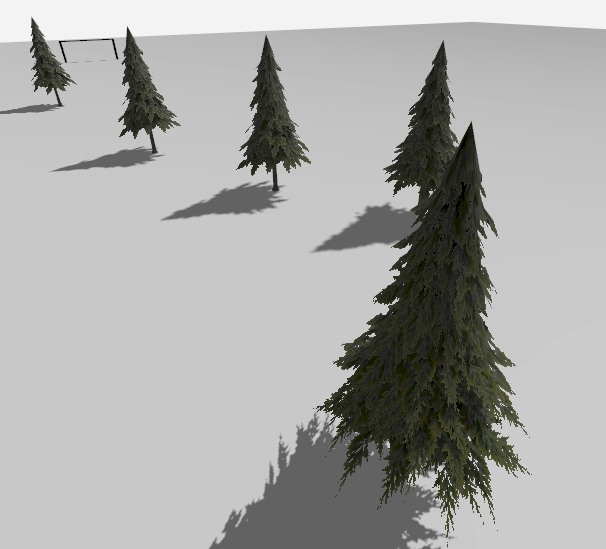
\includegraphics[width = 0.9\textwidth]{images/Track1.png}
        % \captionsetup{justification=centering}
        % \caption{}
    \end{minipage}\hfill
    \begin{minipage}{0.6\textwidth}
        \centering
        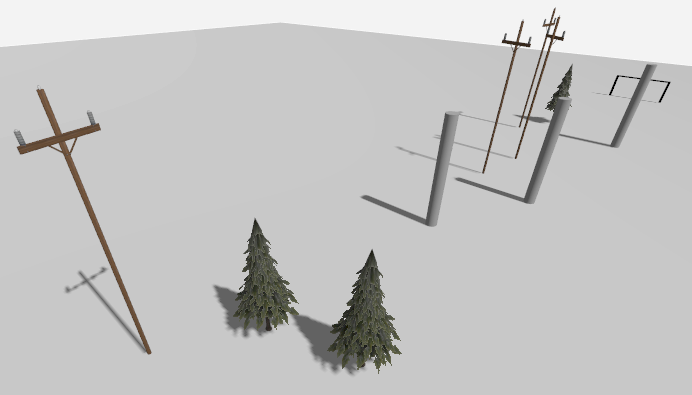
\includegraphics[width = 0.95\textwidth]{images/Track2.png}
        % \captionsetup{justification=centering}
        % \caption{}
    \end{minipage}
    \caption{Przykłady losowo wygenerowanego toru przeszkód dla drona.}
    \label{fig:sceny}
\end{figure}

% Wymaganie 4 - Symulanie DVS - próba prostego podejścia i wykorzystanie v2e
% \vspace{11px}
% \noindent \textbf{Umieszczenie w symulacji kamery zdarzeniowej}
% \vspace{11px}

\subsection{Umieszczenie w symulacji kamery zdarzeniowej}

Pomimo że w bibliotekach środowiska Gazebo dostępnych jest wiele czujników, brakuje gotowego symulatora kamery zdarzeniowej. Dla projektu, w~którym stanowi ona podstawowy element, jest to poważny problem. Jednak dzięki znajomości sposobu działania DVS, można podjąć próbę przybliżenia otrzymywanych z tego czujnika danych za pomocą zwykłej kamery.

W pierwszej kolejności należy umieścić na dronie tradycyjną kamerę. Ta jest dostępna w~Gazebo w~ramach pakietu \textit{gz-sensors}. Rozdzielczość kamery ustawiona jest na $240 \times 180$, co odpowiada rozdzielczości kamery zdarzeniowej dostępnej na rynku i powszechnie używanej (na przykład w~\cite{night_obstacle}) DAVIS240. Wykorzystując ROS-a, stworzony został węzeł, w którym dane z~kamery były na bieżąco odczytywane i~przekształcane do postaci klatek obrazu, a~następnie dalej przetwarzane.

Kamera zdarzeniowa generuje zdarzenia z~każdą zmianą jasności piksela o~stały próg. Najprostszy sposób na ich otrzymanie na podstawie klatek obrazu tradycyjnej kamery może więc wyglądać następująco:
\begin{itemize}
    \item Dwie kolejne klatki obrazu zostają od siebie odjęte (najpierw bieżąca klatka od poprzedniej, a~następnie w~odwrotnej kolejności, aby otrzymać zdarzenia o~dodatniej i~ujemnej zmianie jasności),
    \item Wynikowe obrazy są progowane przy zastosowaniu stałego progu,
    \item Z tak otrzymanych masek odczytywane są wartości położenia $x$ i $y$, dla wszystkich niezerowych pikseli i~zapisywane jako zdarzenie razem z~informacją o aktualnym czasie (ang. \textit{timestamp}) i~polaryzacji (ang. \textit{polarity}).
\end{itemize}

Takie proste podejście zostało zaimplementowane jako osobny moduł symulujący kamerę zderzeniową. Odczytuje on klatki z~kamery, a~następnie symuluje wyjście DVS, publikując przygotowane w~tym celu własne wiadomości (ang. \textit{messages}), zawierające odczytane zdarzenia.

Dodatkowo porównano wyjście symulowane tą metodą z~wyjściem rzeczywistego DVS, za pomocą zbioru danych pochodzących z~kamery zdarzeniowej DAVIS240 \textit{shapes rotation} \cite{dvs_dataset}. Przykładowe porównanie \textit{event frame}'ów jest widoczne na rysunku \ref{fig:frames_comp}. Na klatce, na której reprezentowane są zdarzenia pochodzące z~uproszczonej metody symulowania DVS, piksele (poza szarym tłem) przyjmują wyłącznie wartości skrajne (czarny, biały). Oznacza to, że nie ma różnicy w~czasie ich powstania -- wszystkie zostały wygenerowane w jednym momencie przez odjęcie dwóch klatek obrazu. Dodatkowo na klatce z~v2e widoczny jest szum.

\begin{figure}
    \centering
    \begin{minipage}{0.5\textwidth}
        \centering
        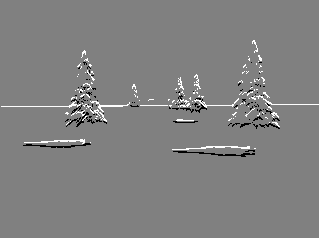
\includegraphics[width = 0.9\textwidth]{images/my_dvs_frame.png}
        \label{gra:my_dvs_frame}
    \end{minipage}\hfill
    \begin{minipage}{0.5\textwidth}
        \centering
        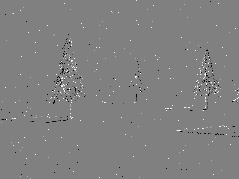
\includegraphics[width = 0.9\textwidth]{images/v2e_frame.png}
        \label{gra:v2e_frame}
    \end{minipage}
    \caption{Przykładowe \textit{event frame}'y dla uproszczonego symulatora DVS (po lewej) oraz v2e (po prawej). Słabo widoczne kształty obiektów na klatce z v2e są wynikiem ograniczonej liczby zdarzeń na jednej klatce i szumu.}
    \label{fig:frames_comp}
\end{figure}

Niestety, mimo że w korzystnych warunkach oświetleniowych i~przy niskich prędkościach względnych obiektów, \textit{event frame} wygląda bardzo podobnie do tego otrzymanego z~rzeczywistych zdarzeń, to tak mocno uproszczone podejście nie może być zastosowane w~celu symulacji DVS. Decyduje o tym kilka czynników:
\begin{itemize}
    \item Jak łatwo zauważyć, w~ten sposób traci się wszystkie z~istotnych zalet kamery zdarzeniowej -- zdarzenia rejestrowane są dokładnie wtedy kiedy klatki obrazu i~z~taką samą czułością, jaką dysponuje tradycyjna kamera,
    \item W przypadku szybciej poruszających się obiektów, liczba klatek na sekundę, jaką rejestruje kamera, może okazać się niewystarczająca -- wtedy zdarzenia pozytywne i negatywne rozdzielają się, co zmniejsza jakość otrzymywanych danych,
    \item W takim podejściu brakuje uwzględnienia szumów, jakie występują w rzeczywistej kamerze zdarzeniowej.
\end{itemize}

Oczywiście nie wszystkie z tych problemów da się całkowicie wyeliminować, ponieważ tak naprawdę czujnikiem zbierającym dane jest zwykła kamera. Można je natomiast ograniczyć przez zastosowanie bardziej dopracowanego systemu symulującego DVS.

% O v2e
\vspace{11px}

Zaawansowane i~dopracowane sposoby na konwersję klatek obrazu z~tradycyjnej kamery na zdarzenia można znaleźć w~literaturze. Kilka z~nich jest zaimplementowanych jako gotowe do użycia narzędzia. Przykładem takiego projektu może być ESIM \cite{ESIM} lub v2e \cite{v2e}.

Do zastosowania w projekcie wybrane zostało v2e, ponieważ oprócz funkcji otrzymywania zdarzeń z wcześniej nagranego filmu, oferuje ono przygotowaną do użycia w~Pythonie bibliotekę, która umożliwia konwersję kolejnych klatek obrazu na zdarzenia w~czasie rzeczywistym. Dzięki temu v2e można zastosować w~węźle ROS-a. 

\textbf{v2e} to \textit{framework} stworzony w~Pythonie, który umożliwia konwersję klatek obrazu ze zwykłej kamery na możliwie realistyczny i~odpowiadający pierwowzorowi strumień zdarzeń. Proces symulacji (na rys. \ref{fig:v2e}) jest wieloetapowy i~obejmuje:
\begin{itemize}
    \item Interpolację klatek, w celu zwiększenia ich częstotliwości, za pomocą narzędzia SuperSloMo \cite{SuperSloMo},
    \item Uwzględnienie logarytmicznej skali, w jakiej działają piksele DVS,
    \item Generację zdarzeń dla każdego piksela na podstawie zmian jasności na poszczególnych klatkach,
    \item Dodanie do sygnału szumów, występujących w rzeczywistych kamerach zdarzeniowych.
\end{itemize}

\begin{figure}
    \centering
    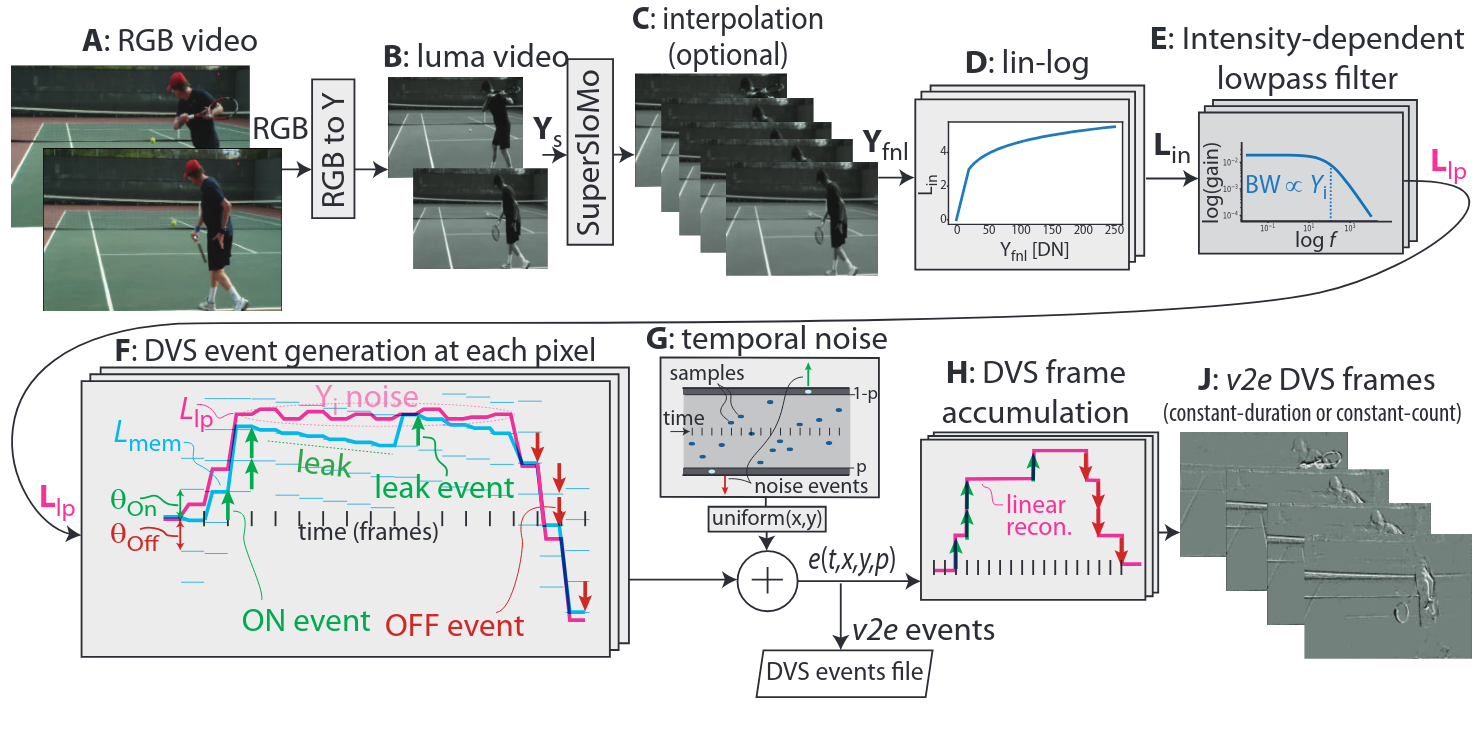
\includegraphics[width=0.85\linewidth]{images/v2e_overview.png}
    \caption{Schemat działania symulacji kamery zdarzeniowej w v2e \cite{v2e}.}
    \label{fig:v2e}
\end{figure}

% Podniesie FPS, żeby poprawić wydajność
Wspomniany emulator ma istotną wadę -- nie pozwala w pełni wykorzystać zalet systemu v2e. Ponieważ narzędzie SuperSloMo \cite{SuperSloMo}, stosowane do interpolacji klatek i~zwiększenia FPS (ang. \textit{frames per second} -- klatki na sekundę) sygnału wejściowego, wymaga zarówno obecnej, jak i~przyszłej klatki obrazu, nie jest możliwe jego zastosowanie bez wprowadzenia dodatkowej latencji.
Wobec tego sposobem na poprawę jakości danych wejściowych kamery jest podniesienie jej FPS. Im większa dynamika sceny (prędkość obiektów), tym bardziej rośnie wymagana wartość FPS. Niestety, wzrost tej wartości znacząco wpływa na wymagania obliczeniowe symulacji i~jakość jej wykonania. Wobec tego, FPS ustawiane jest na najwyższą możliwą wartość, która nie spowalnia działania symulacji zbyt mocno. Testy przeprowadzane były przy wartości $100$ -- zdecydowanie zbyt niskiej dla szybko poruszających się obiektów, jednak należało wziąć pod uwagę ograniczenia sprzętowe.

% \vspace{11px}
% \noindent Poprzednio stworzony moduł został zamieniony na nowe rozwiązanie.

% Tutaj można też napisać o wizualizacji, czyli o agregacji event frame'ów - potem warto opisać terii o DVS

\vspace{11px}

% Poszło do teorii
% Na wyjściu emulatora v2e otrzymywana jest tablica \textit{eventów}, z których każdy zapisany jest jako krotka $(ts, x, y, p)$, gdzie: $ts$, to czas wystąpienia zdarzenia, $x$ i $y$, to jego położenie, a $p$ określa polaryzację. Taka forma danych, chociaż sprawdza się w obliczeniach komputerowych, jest trudna do zrozumienia dla człowieka. Dlatego wyłącznie w celu wizualizacji (ważnej w procesie testowania), zdarzenia są zapisywane jako \textit{event frame}'y z uwzględnieniem ich \textit{timestampów} - tak jak opisane w \cite{Blachut_2023}, przy wykorzystaniu reprezentacji \textit{exponentially decaying time surface}.


\section{Rezultaty}  % Było testy, warto o jakichś też wspomnieć, może z tymi fps-ami, ale głównie to screeny i ich opisy

% Na rysunku \ref{fig:sceny} przedstawiono wyniki uzyskane w etapie opisanym w podrozdziale \ref{subsec:tor}.



% \begin{figure}
%     \centering
%     \begin{minipage}{0.4\textwidth}
%         \centering
%         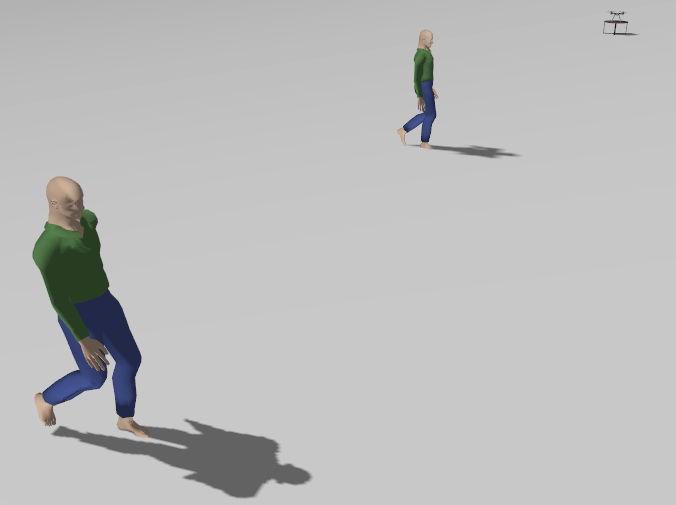
\includegraphics[width = 0.9\textwidth]{images/ludzie.png}
%     \end{minipage}\hfill
%     \begin{minipage}{0.6\textwidth}
%         \centering
%         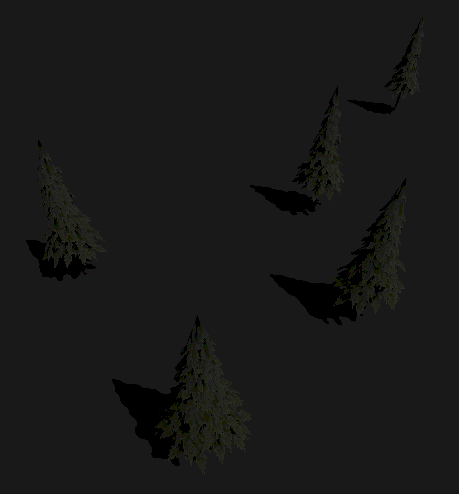
\includegraphics[width = 0.95\textwidth]{images/noc.png}
%     \end{minipage}
%     \caption{Przykłady scen możliwych do stworzenia w celu testów wykrywania przeszkód.}
%     \label{fig:sceny2}
% \end{figure}

% Screen event framów dla pierwszego i drugiego podejścia, można wrzucić błędny screen pierwszego jakby się udało uchwycić, screen widoku z kamery
% Można jeszcze wrzucić coś z testów na shapes.bag

\begin{figure}
    \centering
    \begin{minipage}{0.5\textwidth}
        \centering
        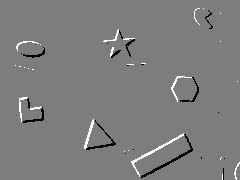
\includegraphics[width = 0.9\textwidth]{images/shapes_slow_my.png}
        \label{gra:my_dvs_shapes}
    \end{minipage}\hfill
    \begin{minipage}{0.5\textwidth}
        \centering
        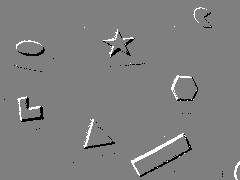
\includegraphics[width = 0.9\textwidth]{images/shapes_slow_org.png}
        \label{gra:real_shapes}
    \end{minipage}
    \caption{\textit{Event frame}'y otrzymane z~klatek obrazu za pomocą uproszczonej metody symulacji DVS (po lewej) i z~danych \textit{shapes rotation} \cite{dvs_dataset} (po prawej), dla małej prędkości ruchu kamery.}
    \label{fig:shapes_slow}
\end{figure}

\begin{figure}
    \centering
    \begin{minipage}{0.5\textwidth}
        \centering
        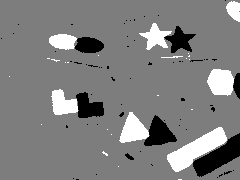
\includegraphics[width = 0.9\textwidth]{images/shapes_fast_my.png}
        \label{gra:my_dvs_shapes_fast}
    \end{minipage}\hfill
    \begin{minipage}{0.5\textwidth}
        \centering
        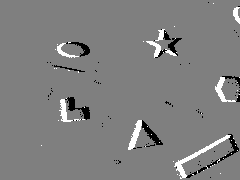
\includegraphics[width = 0.9\textwidth]{images/shapes_fast_org.png}
        \label{gra:real_shapes_fast}
    \end{minipage}
    \caption{\textit{Event frame}'y otrzymane z~klatek obrazu za pomocą uproszczonej metody symulacji DVS (po lewej) i z~danych \textit{shapes rotation} \cite{dvs_dataset} (po prawej), gdy kamera porusza się szybciej.}
    \label{fig:shapes_fast}
\end{figure}


Rysunki \ref{fig:shapes_slow} oraz \ref{fig:shapes_fast} zawierają porównanie uproszczonego sposobu na symulowanie DVS z \textit{event frame}'ami uzyskanymi na podstawie zbioru danych. Szczególnie obserwując \ref{fig:shapes_slow}, można ulec wrażeniu, że prosta metoda jest wystarczająco dobra i klatki niewiele się od siebie różnią. Wystarczy jednak spojrzeć na \ref{fig:shapes_fast}, żeby uświadomić sobie, że uproszczenie to jest zbyt daleko posunięte, żeby ta metoda nadawała się do zastosowania w symulacji. Przy szybkim ruchu kamery obiekty rozdzielają się, tworząc dwa osobne kształty. Generowana jest duża liczba zdarzeń. Negatywnie wpływa to zarówno na złożoność obliczeniową algorytmu detekcji, jak i jego skuteczność -- jedna przeszkoda może być wykryta jako dwie, jej rozmiar i położenie mogą nie odpowiadać rzeczywistemu.

